% !Mode:: "TeX:UTF-8"
% 独立式组网光通信系统的灯组调度

\chapter{独立式组网光通信系统的灯组调度}\label{chap:independent-led-design}
\section{引言}
在上述的分布式组网的架构中,所有的灯组都被调度器控制,从而增大了灯组在房间内的覆盖范围,通过合理的调度方式可以提高了灯组的通信质量,但是这种组网方式没有采用多用户的空分复用技术,系统容量不够高。
本章要研究的系统架构则是独立式的灯组架构,即每个灯组可以独立地控制用户的接入,信息的传输,类似于无线局域网的接入点的概念。基于这种独立式的灯组架构,在多用户的情况下可以采用合理的调度策略,
在保证用户之间没有干扰的前提下,尽可能地提高系统的容量。同时,还需要考虑到用户移动的情形,灯组的调度必须能够适应用户的移动,保证在大量用户运动的条件下,仍然可以获得有效的调度结果。

\section{独立式组网光通信系统分析}\label{sec:analysis}
\subsection{独立式组网光通信系统的调度要求}
为了进行合理的独立式组网灯组调度,首先,需要了解该灯组架构下光通信系统中多用户通信下的调度要求,本文总结了以下四点:

\begin{enumerate}
    \item 在可见光通信系统中,为了满足光照覆盖的要求,通常需要在室内安装多个灯组进行照明,由于每个灯组的覆盖范围有限,
        安装的多个LED灯组一般在室内广泛分布,因此,在使用灯组进行数据传输的过程中,可以使用多个灯组进行协作,从而有效提高用户的数据传输质量;
    \item 在实际通信系统中,用于通信的灯组的覆盖范围较小,且具有明显的定向性。当用户移动出灯组的覆盖范围后,若不采取有效措施,将中断与该灯组的通信。
        因此,对于移动用户而言,调度算法必须能实时地为用户跟踪用户的移动,并选择合适的灯组和资源,保证连接的持续性和稳定性;
    \item 系统容量是衡量多用户光通信系统的一个重要性能指标,因此,在设计合理的调度算法时,必须要将系统容量作为一个重要的优化的目标,保证系统的高性能;
    \item 为了保证灯组调度算法的可实现性,设计的灯组调度算法必须要简单可靠,算法复杂度低,并易于在硬件上实现。
\end{enumerate}

上述的这些需求,其核心都是为了保障多用户通信时系统的整体容量和用户的通信质量。因此,在灯组调度的算法的设计过程中,必须充分考虑到上述提及的对独立式架构下的光通信系统调度要求的分析,形成可靠而有效的灯组调度算法。
下面将先介绍几个本文定义的该架构下的基本通信方式和一些基本概念。

\subsection{多用户复用方式}
为了保证该架构下的多用户的接入和数据通信,系统采用了空分复用和时分复用相结合的复用方式。多个用户可以同时与对应的LED灯组进行数据的传输,这样可以保证获得较大的系统容量。
同时,为了防止用户之间的干扰,系统中的用户被分隔在多个时隙中,以时分的方式进行数据通信。如下图所示

\begin{figure}[htbp]
    \centering
	\includegraphics[width=\textwidth]{figures/chapter-5/IssMultiUserComm.eps}
	\caption{多用户复用方式说明图}
	\label{fig:iss-multi-user-comm}
\end{figure}

上图中,帧的前半部分被用来发送信标帧,管理帧等操作,后半部分则用来进行数据的传输。后半部分被划分为了n个时隙,用于用户的时分通信,在每一个时间片上,多个用户可以同时进行数据通信,如时隙1上,用户1,3和4则可以进行数据的传输。
某个用户可以被分配到多个时隙中进行通信,只要此用户在该时隙上不会造成用户间的干扰即可。

这样,当某一次调度完成后,将会形成上图所示灯组的调度结果。之后的所有的帧都将会按照此结果进行灯组的开关和与用户的通信。

\subsection{用户虚拟小区}
由于在该架构下,各灯组可以独立地传输信息,而根据上述提到的独立式组网光通信系统的特征,为了更好地服务用户,系统可以采用用户周边的灯组来共同协作,进行用户数据的传输。考虑到目前光通信灯组的发送角度都较小,且为了尽可能地保障用户连接的可靠性,本系统采用用户可以接收到的所有灯组给用户发送信息。
这里,我们将可以被用户接收到的所有灯组称作为用户的虚拟小区。灯组以虚拟小区的方式为用户提供光通信数据服务。在一个10个用户,36个灯组的场景中,可以通过下图来描述用户的虚拟小区。

\begin{figure}[htbp]
    \centering
	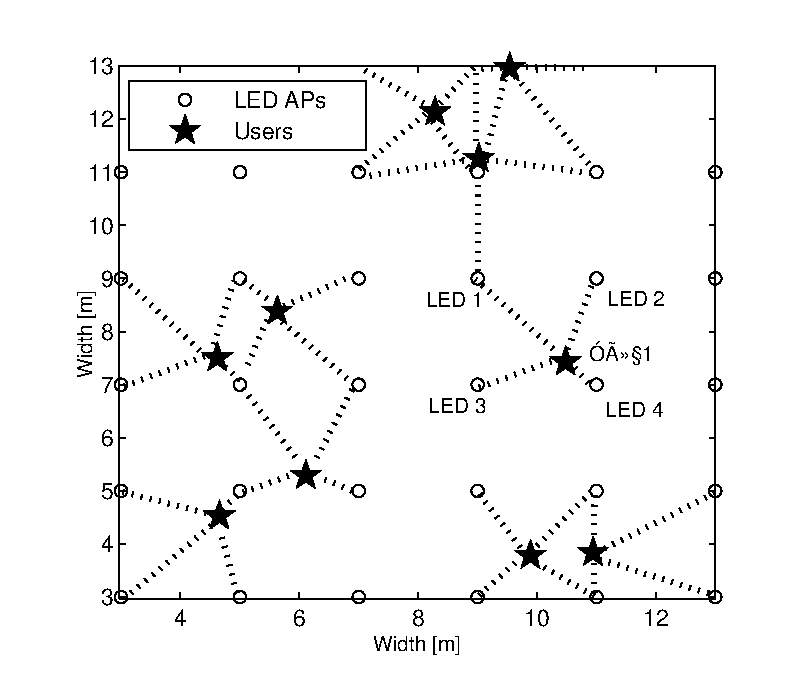
\includegraphics[width=\textwidth]{figures/chapter-5/UserInterference.eps}
	\caption{用户虚拟小区示意图}
	\label{fig:user-interference}
\end{figure}

从上图中,使用星号表示用户的分布情况,使用虚线描绘了各个用户的虚拟小区情况,如LED灯组1,灯组2,灯组3和灯组4将会组成用户1的虚拟小区集合,为该用户服务。同时也可以看到,当两个用户分布较为集中时,其虚拟小区中也就会存在相同的LED灯组,
这也就意味着这两个用户是不能被同时服务到的,必须被分隔在不同的时间片中进行数据传输。具体的用户的干扰问题将在下节描述。

\subsection{用户之间的干扰}
如上所述,当用户的虚拟小区之间存在相同的LED灯组时,则表明用户之间存在相互干扰。本系统为了简化分析,并没有考虑用户之间的干扰的大小,而是设定灯组的调度方案必须能够避免用户之间的干扰。
这样,使用灯组调度算法在每个时隙中选择出来的用户之间必须完全没有相同的LED灯组出现。同样,上述场景下产生的用户间干扰如下图所示。

\begin{figure}[htbp]
    \centering
	\includegraphics[width=\textwidth]{figures/chapter-5/UserInterferenceShow.eps}
	\caption{用户之间的干扰示意图}
	\label{fig:user-interference-show}
\end{figure}

如上图所示,用户1和用户2的虚拟小区中的灯组集合中都包含LED灯组1,因此,用户1和用户2之间存在用户间干扰,为了避免该干扰的产生,这两个用户就不能被同时服务,所以这两个用户需要被调度到不同的时隙中。

\subsection{图论介绍}
图论是数学中的一个分支,它以图作为研究对象。图论中的图是由若干给定的点及连接两点的线所构成的图形,这种图形通常用来描述某些事物之间的某种特定关系,
用点代表事物,用连接两点的线表示相应两个事物间具有这种关系[]。图论的产生和发展主要经历了如下的几个阶段[]。

第一个阶段是从1736年到19世纪中叶。当时图论的焦点主要是比较流行的迷宫问题和游戏类问题。主要最为出名的是著名数学家欧拉解决的哥尼斯堡七桥问题。
欧拉通过图论的方法描述和论证了该问题。第二个阶段是从19世纪中叶到1936年,该段时期图论的发展仍是以游戏类问题为主,如迷宫问题,博弈问题,棋盘行走问题,其中比较著名的问题有四色问题,Hamilton环游世界问题。
图论发展的第三个阶段是在1936年以后,由于计算机和通信网络的不断发展,使得点对点之间的连通性问题不断出现,从而涌现了如最短路问题,稳定性问题等一系列的图论问题,促进了图论的不断发展。
目前,随着计算机的不断运用,图论已经和计算机科学,电子学,信息论不断地结合,并得到了广泛的应用。

图G可以表示为一个二重组合:

\begin{equation}
    G =  < V,E >
\end{equation}

其中$V$是非空有限集合,它的元素被称为结点,而$E$也是一个非空有限集合,其元素被称为边。某条边$e$也可以看作是一个结点的二重组合$<a,b>$,其中$a$和$b$是属于集合$V$。
如果边$e$是有序的,该边就称为有向边,简称为弧,若边$e$是无序的,该边就称为无向边。

每条边都是无向边的图就被称为无向图,而每条边都是有向边的图就被称为有向图。下图分别展示了一个无向图和一个有向图的实例。

\begin{figure}[htbp]
    \centering
	\includegraphics[width=\textwidth]{figures/chapter-5/GraphExample.eps}
	\caption{有向图无向图实例}
	\label{fig:graph-example}
\end{figure}

对于有向图而言,以结点$v$为起点的边数被称为$v$的出度,通常被记为$deg^{+}(v)$,以结点$v$为终点的边数称为$v$的入度,通常被记为$deg^{-}(v)$,而结点$v$的总体度则被定义为上述的入度和出度之和。
对于无向图而言,结点的度则较为简单,就是与该结点相连的所有的边的个数。若所有的结点的度都相等,那么该图就被称为正则图。

给定两个无(有)向图$G=<V, E>$和$G'=<V',E'>$,如果有$V'$包含于$V$且$E'$包含于$E$,则称$G'$是$G$的一个子图。如果此时$G'$不等于$G$,那么$G'$就是$G$的一个真子图。对于一个张图而言,可以生成多个子图。

\section{增量式灯组调度算法}\label{sec:incremental-schdule-scheme}
\subsection{增量式灯组调度算法概述}
灯组的调度需要考虑两个问题,首先是上述的用户优选问题,安排合适的用户在相应的时隙中,利用其虚拟小区中灯组为用户提供服务。在用户的选择时,需要兼顾消除用户之间的干扰和竟可能地增大系统容量。
第二个问题则是用户的移动性问题,当根据当前的所有用户的信息,制定好了最佳的灯组调度策略之后,随着用户的移动,原先的灯组调度策略将有可能不在适合当前用户移动后的场景。
对于第一个问题,我们可以将其看作为一个最优化问题,采用最优化策略来求解。而对于第二个问题,可以采用按照一定频率反复运行灯组调度算法来不断地根据当前场景进行灯组调度。但是这样做,会带来高复杂度和运算量的问题。

本文提出了一种增量式调度算法来解决独立式灯组组网光通信系统下的移动性多用户灯组调度问题,算法主要包含两个部分,全局调度算法和局部调度方法。
其中全局调度算法采用图论的方法对用户位置及用户间干扰进行建模,综合考虑到所有用户的情况,力图达到一个全局最优或者接近最优的系统容量,但是全局调度算法具有复杂度高的缺点。
而局部调度算法则是在全局调度算法结果的基础上,考虑到当前发生移动的用户,采用简单的方案为其重新安排合适的灯组,并协调好与其他灯组之间的关系,在没有过分损失系统容量的情况下适应移动用户的运动,并减低用户的运算量。

增量式调度方案由长时间周期调度的全局算法和短时间周期调度的局部算法组成,即运行一次全局调度,再运行多次局部调度,并重复执行,可以综合两种调度方案的优点,克服只使用全局最优算法导致的运算量大的缺陷,
在获得较好的系统容量的前提下,显著降低系统调度的运算量。下面将会分别介绍两种调度子算法,并详细地对上述的两种子调度算法进行分析。

\subsection{全局调度方法}
全局的调度算法考虑到所有用户当前可使用的灯组情况,以系统容量作为优化目标,通过建立带权重的无向图对该问题进行建模,并提出了比较完善的调度方案。
该算法在分析所有用户信息的基础上,将用户分配到合适的时隙上,消除了用户之间的干扰,并保证了较优的系统容量。

\subsubsection{用户优选问题的建模}
首先需要定义一些系统的参量,如上文所说,在每个用户在通信时,为了获得可靠的通信效果,可以使用虚拟小区为其提供通信协作,因此这里定义为用户$u_{i}$服务的虚拟小区为$VC_{i}$。

为了最大化系统的容量,本文定义了以下的系统效用函数:

\begin{equation}
    \sum\limits_{i = 1}^K {{U_i}({{\bar r}_{i,k}})}
\end{equation}

其中,$U_i()$是一个用于衡量用户$u_{i}$吞吐量的效用函数,${\bar r}_{i,k}$是用户$u_{i}$在时隙$i$前计算出的平均速率,定义为:

\begin{equation}
    {\bar r_{i,k}} = (1 - \frac{1}{{{T_c}}}){\bar r_{i,k - 1}} + \frac{1}{{{T_c}}}{r_{i,k - 1}}
\end{equation}

其中,$T_{c}$表示为比例系数,该值可以决定在前一个时隙中用户的速率占用户的平均速率的比例。

假设第$k$个时隙中的所有用户可达速率集合的向量定义为

\begin{equation}
    \overrightarrow {{r_k}}  = {[{r_{1,k}},{r_{2,k}},...,{r_{K,k}}]^T}
\end{equation}

其中,$r_{i,k}$指的是在时隙$k$上用户$u_{i}$可以获得的速率。根据基于梯度的调度框架[],调度的主要目标就是在梯度的方向上选择合适的$\overrightarrow {{r_k}}$,因此,最优化系统容量的问题转化为:

\begin{equation}
    \max \sum\limits_{i = 1}^K {{{U'}_i}(\overline {{r_{i,k}}} )} {r_{i,k}}
\end{equation}

本文采用了一个较为典型的效用函数,如下所示:

\begin{equation}
    {U_i}(\overline {r}_{i,k}) =
    \begin{cases}
        \alpha^{-1} {\overline {r}_{i,k}}^\alpha ,  & \alpha \le 1 \mbox{and} \alpha \ne 0 \\
        log(\overline {r}_{i,k}),                   & \alpha = 0
    \end{cases}
\end{equation}

其中,$\alpha$表示公平系数,代表用户间可达速率的公平程度,将()代入(),于是问题也就被转化为:

\begin{equation}
    \max \sum\limits_{i = 1}^K {{{\overline {r}_{i,k} }^{\alpha  - 1}}{r_{i,k}}}
\end{equation}

可见,当前的目标函数将会受到参数$\alpha$的影响,不同的$\alpha$值将代表着不同的公平性,为了满足系统的要求,这里较为简单地设置$\alpha$为0,
这样,目标函数就转变为:

\begin{equation}
    \max \sum\limits_{i = 1}^K {\frac{{{r_{i,k}}}}{{\overline {r}_{i,k} }}}
\end{equation}

上述的目标函数则是调度算法在每个时隙选择合适的用户时需要考虑的目标,同时为了防止用户之间干扰的产生,需要保证每个时隙中的用户之间没有公用的灯组,
所以对于上述的目标函数,还需要引入一定的约束条件,时隙间用户不存在干扰,各用户的虚拟小区间不存在公共的灯组等,所以系统的优化模型就转变为:

\begin{equation}
\begin{aligned}
    \max\quad & \sum_{i=1}^{K}\frac{r_{i,k}}{\overline{r}_{i,k}} \\
    s.t. \quad & I_{i} = 0,\; i=1,...,K \\
        & VC_{i} \cap VC_{j} = \emptyset  i,j= 1,...,K and i \ne j  \\
        & \bigcup_{i = 1}^K V{C_i} \subseteq A
\end{aligned}
\end{equation}

其中,$I_{i}$代表用户 接收到的干扰信号,集合$A$代表所有的灯组集。

对于$r_{i,k}$,可以用香农公式展开。$r_{i,k}$与用户$u_{i}$在$k$时刻的接收信号功率有关,而由于系统中各个灯组会周期性地发送信标帧来使用户获得当前的灯组信息,
而且信标帧发送的周期较短,两次信标帧之间用户几乎不会发生移动,因此,用户侧可以采用上一次接收到的信标帧的接收功率来近似表示用户当前时隙的接收信号,即

\begin{equation}
    {h_{i,j}}{P_{ot}} \approx {P_{recvj}}
\end{equation}

最后,将$r_{i,k}$按公式展开并带入公式(),可以得到用户优选的系统最优化模型:

\begin{equation}
\begin{aligned}
    \max\quad & \sum_{i=1}^{K}\frac{log_{2}(1+\frac{{\sum_{LA_{j} VC_{i}}RP_{recvj}}^2}{I^2+\delta^2})}{\overline{r}_{i,k}} \\
    s.t.\quad & I_{i} = 0,\; i=1,...,K \\
        & VC_{i} \cap VC_{j} = \emptyset  i,j= 1,...,K and i \ne j  \\
        & \bigcup_{i = 1}^K V{C_i} \subseteq A
\end{aligned}
\end{equation}

\subsubsection{系统模型的解决}
针对上述的最优化问题,因为离散问题的全局最优化问题很难直接解决,本文运用图论的方法将该问题使用图论进行了重新的描述,并采用相应的算法对该图论问题进行了求解。

由于用户在灯组下的布局很容易用一个无向图进行表示,同时用户之间的干扰也可以用图论中两个节点是否存在连接线来表示,所以,本文采用了一个带权重的无向图来对上述最优化问题进行了重新的建模。
首先,需要可以定义一些参数,$G(V,E)$表示建立的用户干扰图,$V(G)$表示图G中的顶点集,$E(G)$表示图$G$中的边集。$v_{i}$表示在点集$V_{G}$中的一个节点,$N(v_{i})$表示该节点的相邻节点集,
$d(v_{i})$表示节点$v_{i}$的度,也就是相邻节点集$N(v_{i})$中节点的个数。在用户图上对于每个节点增加一个权重值,就构成了带权重的无向图$G^{w}(V,E)$。干扰图中的顶点$v_{i}$代表场景中的某一个用户,
而干扰图中的在边则依据用户之间是否存在干扰,当两个用户之间存在干扰时,图中的两个顶点之间也就存在一条边,否则两点之间没有连线。同时根据前一节分析的调度目标函数,
这里按照式()在时隙$k$时设置干扰图中各个顶点的权重值。

\begin{equation}
    {p_{i,k}} = \frac{{{r_{i,k}}}}{{\overline {r}_{i,k} }}
\end{equation}

对上述给出的多用户在多个灯组下的通信场景按照上述的图论的方法进行建模,可以得到描述该系统用户之间干扰的干扰图如下:

\begin{figure}[htbp]
    \centering
	\includegraphics[width=\textwidth]{figures/chapter-5/InterferenceGraph.eps}
	\caption{用户干扰图}
	\label{fig:interference-graph}
\end{figure}

图中,五角星则表示的是场景中的用户,之间的连接线表示的是用户之间存在干扰。例如,用户1和用户4之间是存在干扰的,在同一个时隙下不能被同时选中,用户1和用户6之间是不存在干扰的,可以同时进行数据通信。

经过上述图论的描述之后,问题被转变为如何在这个带权重的无向图中找到一组顶点,使得任意两个顶点之间没有边,同时该组顶点的权重值之和最大。该组顶点的集合可以被记为最大权重顶点集。参考文献[],使用了贪心算法可以很好地解决这个问题。
在使用贪心算法中,依据的思想是如果图中某一顶点的度越大,该顶点干扰的其他用户也就越多,因此该顶点也就越不应该被选中。所以系统以$p_{i,k}^{'}=\frac{p_{i,k}}{d(v_{i}+1)}$作为标准来进行某一时隙激活用户的选取。每次选取$p_{i,k}^{'}$值最大的顶点,
并将该顶点和图中与该顶点相邻的顶点集合去掉,重复上述过程,直到图中的顶点全部被选择完成为止。具体的基于图论的灯组选择算法为:

%
%算法图
%

上述的基于图论的灯组选择算法可以保证在一个时隙中选择出合适用户,但为了保证每个用户在此次调度中都能够被服务到,本文使用了比例公平算法,从而保证能在多个时隙中服务完成所有的用户。

比例公平算法的目的是,为了保证在上一个时隙被服务过的用户就只能获得较小的权重,而上一时刻没有被服务的用户可以获得较高的权重,从而,可以将所有用户较好地安排在多个时隙中。
因此,系统在调度完成一个时隙之后,会按照式()重新更新当前的用户图上各节点的权重,然后再次按照上述基于图论的灯组选择算法选择另外一组用户,直到所有的用户都被服务过。

根据上述的描述,全局调度算法可以总结为以下步骤:

\begin{enumerate}
    \item 各灯组每隔一段时间会定时发出的beacon信息,用户将会记录下beacon信息的接收功率和发送的灯组号,并上报给光通信中的调度器;
    \item 调度器利用上报的信息形成用户之间的干扰图,并为各阶段计算出相应的权重值;
    \item 根据干扰图各节点的权重,依据贪心算法分析出当前时隙可被激活的用户;
    \item 更新干扰图中的节点权重信息;
    \item 重复(3)直到所有的用户均被服务过;
    \item 得到灯组的全局调度结果。
\end{enumerate}

\subsection{全局调度方法}
由于场景中用户的移动性,使得全局调度产生的灯组调度方案在一段时间后将不再适应于用户当前的位置,具体点说,则是用户的移动导致了用户当前的虚拟小区将不再是全局调度时刻的虚拟小区。
因此,系统采用局部调度方法根据当前用户上报的信息,选择出需要进行局部调整的用户,采用了回溯算法,为移动用户更新合适的灯组资源,进而保障通信中用户的移动性。局部调度算法可以按照以下三部分进行。

\subsubsection{运动用户集合}
运动用户集合的划分主要通过用户的上报的灯组信标帧的情况进行划分,由于系统的每个灯组在超帧时间内都会发送信标帧来广播自身的信息,所以当用户接收到周期性发送的灯组信标帧之后,就会将接收到的灯组的编号反馈给系统调度器,该组灯组的编号也就是当前可以为该用户提供服务的灯组集合。
当调度器一段时间内统计到某个用户的可用灯组信息发生了变化后,就将该用户放入到运动用户集合(moving user set,MUS)中,等待进行后续的调度操作。

\subsubsection{子图内用户间干扰}
局部调度是在全局调度的基础上进行的,当全局调度完成之后,系统将会获得全局调度的调度信息,如具体时隙中使用哪些灯组服务哪些用户。因此,当已知了移动用户的集合之后,可以同样从全局调度中的图论的角度出发。
全局调度会把所有的用户划分在若干个调度子图中,即每一个调度的时隙中的用户及其之间的关系形成一个调度子图。在子图中,由于全局调度完成后会保证子图中的用户之间是没有干扰的,因此调度完成之后的子图中各个结点之间是没有连线的,
同样,上述实例中进行了全局调度后的子图划分如下所示。

\begin{figure}[htbp]
    \centering
    \subfloat[第一个子图]{
        \label{fig:slot-1-before-move}
        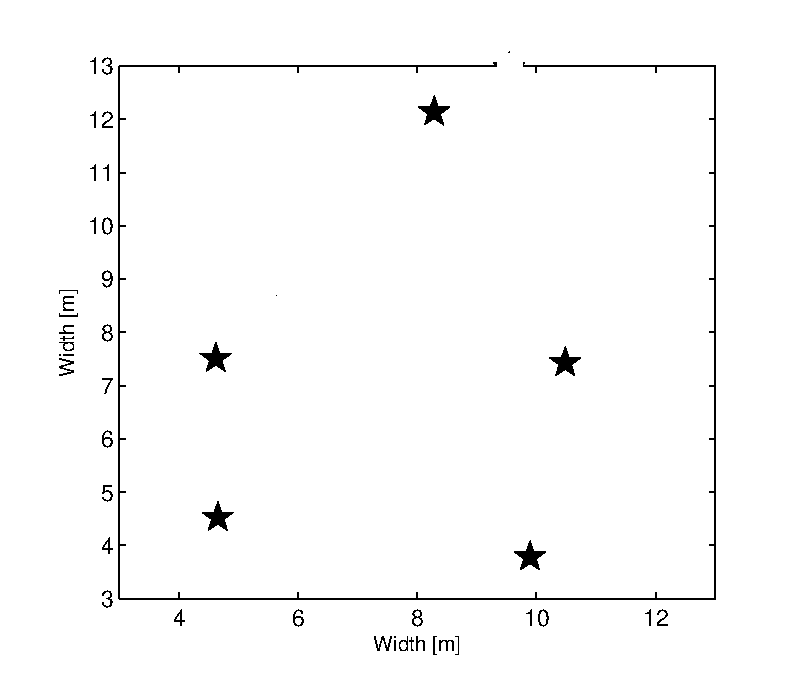
\includegraphics[width=0.5\textwidth]{figures/chapter-5/UserBeforeMove1.eps}
    }
    \subfloat[第三个子图]{
        \label{fig:slot-3-before-move}
        \includegraphics[width=0.5\textwidth]{figures/chapter-5/UserBeforeMove3.eps}
    }
    \caption{用于运动前的子图情况}
    \label{fig:slot-before-user-move}
\end{figure}

在一段时间之后,当用户位置发生了改变,会使得用户之间再次形成干扰,这样的干扰当然可以再一次使用全局调度来解决,但如上分析,那将会耗费较大的调度时间。这里首先可以充分利用全局调度带来的多子图的优越性,全局调度能够将距离较近,容易形成干扰的两个用户分隔在不同的时隙中,
从而使得用户移动带来的影响分散到各个子图中。因此,当用户移动后,我们只需要去关注和解决子图中的用户间干扰即可。如下图所示,当用户7发生了移动,则会在子图1和子图3中发生用户间的干扰,局部调度就是要去解决这两个子图中的干扰即可。具体的子图中干扰解决方案将在下节中进行讨论。

\begin{figure}[htbp]
    \centering
    \subfloat[第一个子图]{
        \label{fig:slot-1-after-move}
        \includegraphics[width=0.5\textwidth]{figures/chapter-5/UserAfterMove1.eps}
    }
    \subfloat[第三个子图]{
        \label{fig:slot-3-after-move}
        \includegraphics[width=0.5\textwidth]{figures/chapter-5/UserAfterMove3.eps}
    }
    \caption{用于运动前的子图情况}
    \label{fig:slot-after-user-move}
\end{figure}

\subsubsection{移动用户最优时隙选择}
在考虑如何处理移动用户可能带来的用户间干扰前,可以先考虑一下如下方面问题。首先,由于在全局调度后某个用户有可能会在多个子图中出现,它的移动也可能引起多个子图内的用户间干扰。其次,某个用户的移动可能会导致该用户适合于原先不存在该用户的子图,因此,对于运动用户的调度,
不应该仅仅着眼于它当前分配的子图中,也应该考虑其在其他子图中出现的可能性。

在解决子图干扰时,所有非运动用户仍然分配在全局调度所分配的子图中,系统通过对运动用户集合中的用户进行调度,在兼顾系统容量的同时,保证运动用户可以获得较好的调度灯组,完成系统的局部调度,这种方式也将大大减小局部调度所需要的运算量。

这里,可以分两种情况来讨论用户移动在全局调度基础上对系统造成的影响。一种情况是某个用户的移动在子图内都没有造成子图中用户间的干扰,对于这种情况,系统可以直接将全局调度中为该用户服务的灯组更改为该用户当前的虚拟小区中的灯组即可。另一种情况则是当用户的移动在某一个子图中造成了子图中用户间的干扰,
这里就需要对该用户的可存在性进行判决。若要使得用户可以存在于子图中,就必须将用户放入子图中时,关闭该时隙内所使用的所有灯组中与该用户虚拟小区中相同的LED灯组,这种关闭相同灯组的方式可以消除用户间的干扰,但是当移动用户与它所在时隙中其他用户的LED灯组的重复率过高时,会严重降低系统容量。
因此,为了保障系统容量,对于移动用户在子图中可存在性判决的依据是用户在子图中的存在将导致子图的容量值的变化。系统定义的一个子图容量变化值如下式

\begin{equation}
    \Delta {C_{ij}} = {C_{aij}} - {C_{bij}}
\end{equation}

其中,$\Delta {C_{ij}}$表示的是在子图$SG_{i}$中添加用户$u_{j}$后引起的子图容量的变化,$C_{bij}$和$C_{aij}$表示的是在加入用户$u_{j}$之前和之后的子图的系统容量,定义子图k中的系统容量计算公式为:

\begin{equation}
    {C_k} = \sum\limits_{i = 1}^K {{{\log }_2}(1 + \frac{{{{(\sum\limits_{L{A_j} \in V{C_i}} {R{P_{recvj}}} )}^2}}}{N}))} {\kern 1pt} {\kern 1pt} {\kern 1pt} {\kern 1pt} {\kern 1pt} {\kern 1pt} {\kern 1pt} {\kern 1pt} {\kern 1pt} {\kern 1pt} {\kern 1pt} {\kern 1pt} {u_i} \in A{U_k}
\end{equation}

其中$AU_{k}$表示的是子图中被激活的用户。

当$\Delta {C_{ij}}$为正时,则表明把运动用户存在在此子图中时,对获得系统容量的增加有利,当该值为负时,则表明用户在此子图的存在,
将会对其他用户造成较为严重的干扰,不能保证很好的系统容量,该用户不应该分配在该子图中。

于是,根据上述的算法和移动用户自身的特点,对运动用户集合中的每个用户,判断其干扰产生的影响,并为其选择合适的调度灯组,
从而获得较优的灯组调度结果。综上所述,局部调度主要分为如下几个步骤:

\begin{enumerate}
    \item 根据用户上报信息,根据灯组集的改变情况,组成局部调度用户集;
    \item 调度器利用上报的信息形成用户之间的干扰图,并为各阶段计算出相应的权重值;
    \item 根据干扰图各节点的权重,依据贪心算法分析出当前时隙可被激活的用户;
    \item 更新干扰图中的节点权重信息;
    \item 重复(3)直到所有的用户均被服务过;
    \item 得到灯组的全局调度结果。
\end{enumerate}

\section{仿真实验及结果分析}\label{sec:iss-simulatioon-result}
为了对提出的增量调度的算法进行分析,本文在NS2平台上进行了独立式灯组光通信场景模型的建立和仿真,模拟了用户在用户过程各种灯组的调度过程。仿真中的场景和上述的实例一样,设置了6*6个灯组和10个用户,灯组被规则地分散放置在房间内,
用户的位置则是随机均匀分布在用户接收平面上,仿真中需要设定具体的光通信参数,如灯组的属性,干扰的具体参数等,其具体数值列表如下:

\begin{table}[htbp]
    \caption{独立式灯组调度仿真参数表}
    \label{tab:iss-simulation-param}
    \centering
    \begin{tabular}{llll}
        \toprule
        参数     & 数值 & 参数 & 数值 \\
        \midrule
        d        & 2m                & h           & 2.2m \\
        A        & $0.785mm^{2}$       & $P_{ot}$      & $3600*30mw$ \\
        $T_{k}$    & 300k              & $\Phi_{1/2}$  & 70deg. \\
        $\eta_{c}$ & $1.12*10^{-6}F/m^2$ & R           & $0.54A/W$\\
        G        & 10                & $I_{bg}$      & $5.1*10^{-3}A$ \\
        $\Gamma$   & 1.5               & $I_{2}$       & 0.562 \\
        $I_{3}$    & 0.0868            & B           & 100MHz \\
        $g_m$      & 0.03S \\
        \bottomrule
    \end{tabular}
\end{table}

为了考察本文的增量式调度算法对移动用户和系统性能的影响,在仿真中主要从移动用户的接收信噪比的情况和调度对系统容量的影响来进行系统的分析。

这里定义用户的接收信噪比为:

\begin{equation}
    SNR = \frac{{\sum\limits_{i = 1}^N {{{(\sum\limits_{A{P_j} \in V{C_i}} {{h_{ij}}{P_{ot}}R} )}^2}} }}{N}
\end{equation}

其中,$N$表示的是该用户虚拟小区中的灯组的个数。而在一个时隙中用户的系统容量为:

\begin{equation}
    capacit{y_m} = \sum\limits_{i = 1}^K {{{\log }_2}(1 + \frac{{{{(\sum\limits_{A{P_j} \in V{C_i}} {{h_{ij}}{P_{ot}}R} )}^2}}}{N})}
\end{equation}

其中$K$表示该时隙中的用户的个数。则在整个调度过程中系统的总的系统容量为:

\begin{equation}
    capacity = \sum\limits_{m = 1}^M {capacit{y_m}}
\end{equation}

在仿真中,为了检验本文所提出的增量式调度算法的性能,设置了两种对比算法,即高频度的全局调度和低频度的全局调度,其中高频度的全局调度算法由于能够及时根据所有用户的位置进行灯组调度,可以看作为接近最优系统容量的调度方法。而把低频度的全局调度的调度时间间隔设置为10s,和采用了间隔10s调度一次的全局调度和间隔1s调度一次的局部调度相结合的增量式调度方法相比,
低频度的全局调度算法可以看作为只是用了全局调度而没有使用局部调度算法的增量式调度。

\subsection{不同的用户移动速度对用户SNR分布的影响}
仿真中,将10个用户初始随机地分布在接收平面上,首先使得一个用户进行移动,为了检查算法对移动用户的支持,本文采用了cdf曲线来考察用户的接收信噪比的分布情况。分别仿真了用户在1m/s情况下的高频度全局调度和低频度全局调度的用户信噪比分布情况和用户在0.5m/s,1m/s和2m/s下使用本文提出的增量式调度方法的接收信噪比分布。
其仿真结果如下图所示。

\begin{figure}[htbp]
    \centering
	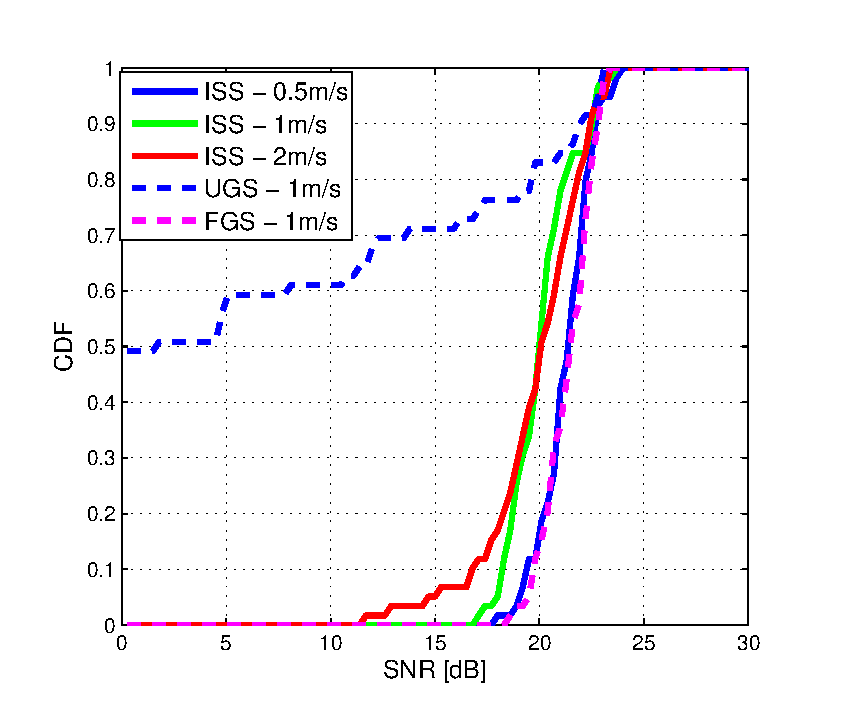
\includegraphics[width=\textwidth]{figures/chapter-5/Speed2Snr.eps}
	\caption{用户移动速度对用户SNR分布的影响}
	\label{fig:speed-2-snr}
\end{figure}

从上图中可以看出,短频度的全局调度算法由于不能很好地对用户的移动性提供支持,当用户运动后,由于系统没有能够及时地进行调度,导致为该用户服务的灯组还是原先设定的LED灯组,从而导致系统的接收信噪比的取值较为分散,在0-24dB均有分布。而与之相比,由于高频度的全局调度能够实时地进行用户LED灯组的调度,
所以也就能确保用户获得很好的信噪比的分布,其用户信噪比都集中分布在18-23dB附近。而本文提出的增量式调度算法,其接收信噪比远好于低频度的全局调度,并当用户的速率较低时,其信噪比分布接近于高频度的全局调度的分布。同时我们可以看到,当用户的移动速率变高时,用户的信噪比cdf分布也就越宽。
这是因为,随着用户的移动速率的逐渐增加,使得移动用户移动到接收信号差的区域的几率增加,从而导致用户低信噪比出现的概率增加。图中的数据表明,在正常的用户移动速率下,用户的信噪比分布较为平稳,能基本满足高速数据通信的需求。

\subsection{不同的接收视场角对用户SNR分布的影响}
由于用户的接收视场角对系统的调度有着重要的影响,不同的接收视场角使得用户的虚拟小区中灯组集的差距较大,也导致不同的用户间干扰的产生。
因此,本文仿真了接收视场角在40度,45度,50度和55度这四种情况下,移动用户的接收信噪比的cdf分布情况,其仿真结果如下图所示:

\begin{figure}[htbp]
    \centering
	\includegraphics[width=\textwidth]{figures/chapter-5/Fov2Snr.eps}
	\caption{接收视场角对用户SNR分布的影响}
	\label{fig:Fov-2-Snr}
\end{figure}

从图中可以看到,用户的接收视场角对于用户的接收功率的影响较大。随着用户的接收视场角的增大,其信噪比也就越高。这是因为,$FOV$的增加,将会使得可以为该用户服务的灯组的个数也就随之增多,这样对于单个用户来说,其接收信噪比也就增大了,
但是,FOV的增加将会导致用户的虚拟小区的重叠灯组的增多,也就意味着用户间的干扰增加,这样,在进行增量式调度中的全局调度时,就会需要更多的时隙才能将所有用户服务完,也会给后续的局部调度增加复杂度。因此,在本文的算法中,可以在满足用户的信噪比需求的前提下,尽可能选择较低的FOV值。

\subsection{不同的用户数对各调度算法下系统容量的影响}
在室内可见光通信中,用户的规模对系统的调度有着至关重要的影响。为了讨论在不同的用户数的情况下,本文的调度算法对系统性能的影响,进行了如下的仿真。
在仿真中,同样设置场景中存在一个用户进行随机移动,其他用户不运动,并调整不同的用户数量进行仿真,仿真结果如下图所示。

\begin{figure}[htbp]
    \centering
	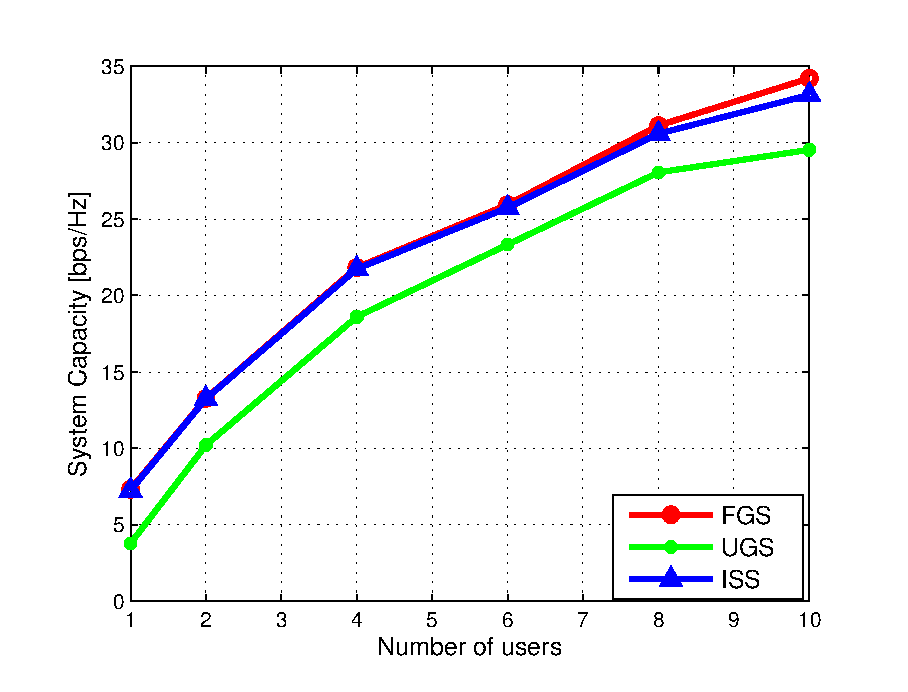
\includegraphics[width=\textwidth]{figures/chapter-5/Usernum2Capacity.eps}
	\caption{用户数对系统容量的影响}
	\label{fig:usernum-2-capacity}
\end{figure}

从图中可以看出,显然随着用户数的不断增加,系统的容量值也不断提高。在当前仿真的一个用户运动的情况下,本文提出的增量式调度算法的系统容量的指标非常贴近于高频度的全局调度算法得到的系统容量曲线。这是因为,本文提出的增量式调度算法不管是在全局调度阶段还是在增量式调度阶段,都很重视对系统的系统容量的影响,
系统容量也是调度算法优化的一个重要指标,在局部调度阶段,虽然用户间的干扰的消除会降低系统的容量,但其对系统容量的影响也是被控制在很小的范围内。因此,本文所提出的增量式调度算法拥有很好的系统容量性能。而低频度的全局调度算法与之相比,在系统容量方面与上述两种算法有差距很大。这是因为进行低频全局调度后,
调度周期内的用户通信质量并不是得以保证,移动中的用户很有可能就会移动出原有的灯组调度范围中,从而带来整体通信性能的下降。上述仿真中假设的是单个用户运动,若场景中存在多个用户运动时,在不同的用户数下系统容量的区别将会更加明显,而由于增量式调度算法中含有针对于移动用户的局部调度算法,因此其调度性能还是可以得到保证的,
具体针对多移动用户的仿真将在下文中详细分析。

\subsection{不同的移动用户数对各调度算法下系统容量的影响}
上述的仿真只提供了一个移动用户的场景,而保障多个用户的移动性时本文算法研究的重要方向,为了研究算法在不同移动用户数目下的系统性能,
本文分别使用三种调度算法,在总的用户数目为10,移动用户的数目分别设定为0到10的情况下,进行了仿真研究。得到的仿真结果如下图所示:

\begin{figure}[htbp]
    \centering
	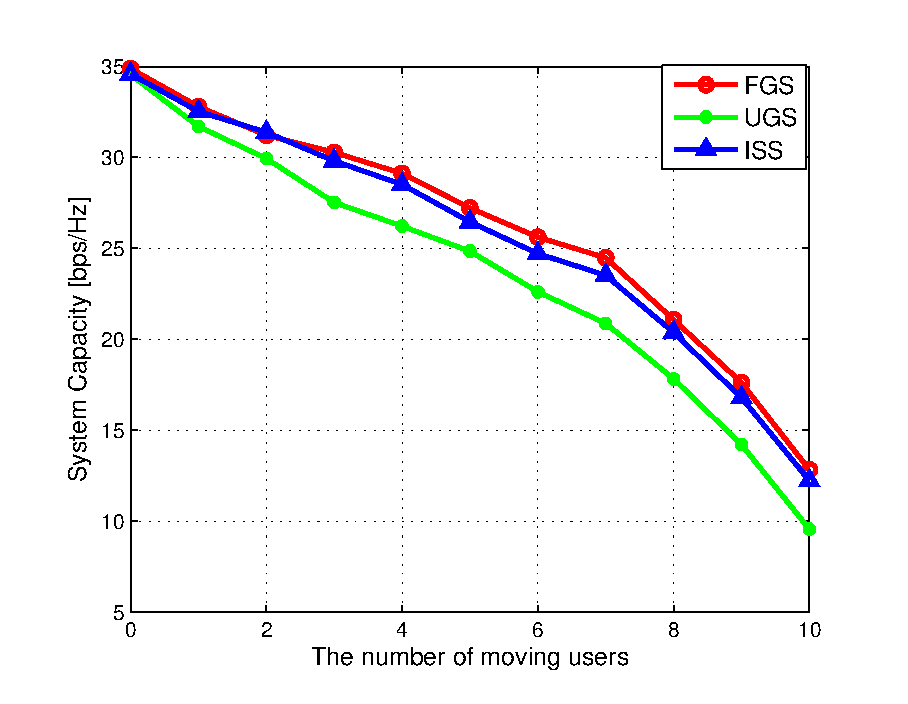
\includegraphics[width=\textwidth]{figures/chapter-5/MovingUserNum2Capacity.eps}
	\caption{移动用户数对系统容量的影响}
	\label{fig:moving-user-num-2-capacity}
\end{figure}

从上图可知,随着移动用户数目的不断增加,三种调度算法的系统容量都呈现不断下降的趋势,这是因为用户移动会导致用户的平均接收信噪比降低,进而影响到整体系统的速率。其中最上面的曲线为采用高频度全局调度的系统容量结果,
因为高频度的全局调度会最大限度得保障系统的所有用户的调度结果最优,使得系统性能接近于理论最优值,所以其系统容量的表现是最好的。低频度的全局调度由于其调度周期的局限性,在多个用户移动的情况下,其系统性能的差距变得非常明显,远低于其他两种算法。
而增量式调度算法由于在局部调度阶段充分考虑到移动用户对系统容量的影响,并为其进行了较优的灯组调度,从而使得在多个移动用户的情况下,增量式调度算法的表现仍然能非常地接近于类似最佳表现的全局调度,也远优于低频度的全局调度。
这说明本文提出的增量式调度算法能够适应存在多个移动用户的调度场景,并能达到较为理想的系统性能要求。

\subsection{不同的移动用户数对各调度算法下复杂度的影响}
在室内可见光通信系统中,对系统调度算法进行分析时,除了对算法的整体调度性能进行分析之外,还需要考虑算法在调度复杂度上的表现。
良好的调度算法应该具有较低的复杂度和较好的硬件可实现性,因此为了比较以上三种算法在算法复杂度上的差异,
本文通过仿真比较了三种算法的总的运算时间。这里的总的运算时间是指在一次仿真中调度算法所使用的平均运算时间。仿真时的参数设置和上一节的设置一样,仿真后的结果如下图所示。

\begin{figure}[htbp]
    \centering
	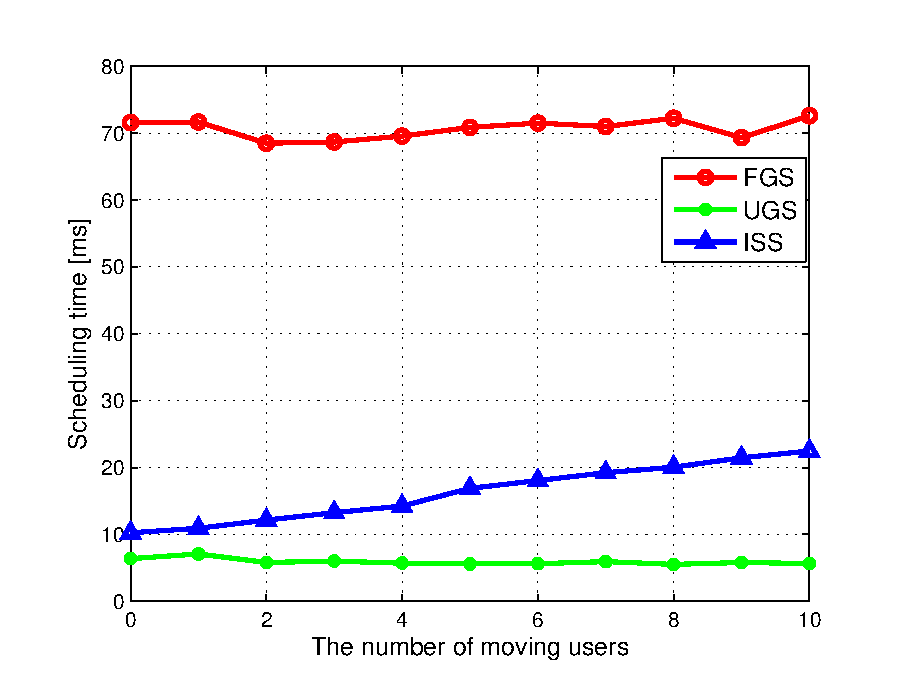
\includegraphics[width=\textwidth]{figures/chapter-5/MovingUserNum2Complexity.eps}
	\caption{移动用户数对调度复杂度的影响}
	\label{fig:moving-user-num-2-complexity}
\end{figure}

从上图中可知,高频度的全局调度由于需要短时间间隔的针对所有用户的调度,所有其调度所花费的计算时间也是最长的,而本文所提出的增量式调度方法远优于高频次的全局调度算法,这是因为高频次调度算法需要不断地进行复杂度很高的全局调度操作,
而增量式调度算法在一次全局调度后只需要复杂度较小的多次局部调度来进行灯组调整即可,所以运算的复杂度也大为降低,其在10个移动用户的情形下,调度所需要的运算量只有高频次全局调度算法的30\% 左右。
同时,对于低频度的全局调度,由于其不含有局部调整,全局调度的周期又比较长,因此它的运算复杂度也是最低的。综上分析可以知道,本文提出的增量式调度方法在系统调度的运算复杂度方面的性能是较优的。


\section{本章小结}
本章主要研究了在独立式灯组布局的条件下灯组的调度策略。独立式灯组是指各个灯组的数据传输都是独立进行的,相互之前不相互影响。这种组网方式下的灯组可以进行空分复用,从而提高系统的容量。本章首先介绍了独立是灯组的概念,并提出了在该架构下用户的虚拟小区的概念和多用户用户间干扰的产生。
对于该网络结构,本章提出了一种增量式灯组调度算法来进行灯组的最优化的调度。该增量式灯组调度算法可以分为两个阶段,第一个阶段是采用的是全局调度算法,该算法的目的是考虑当前网络内所有用户的状态,并基于图论的算法,给出一种近似最优的灯组调度结果,将所有用户安置在不同的时隙中进行通信,
并保证在同一时隙中没有用户间的干扰产生。第二个阶段是在全局调度周期内,采用多次低复杂度的局部调度算法,只处理当前运动中的用户,考虑移动用户对当前系统中用户间干扰产生的影响,并进行相应的灯组调度结果调整,从而使得灯组的调度适合移动用户的运动。本章提出的增量式调度算法,通过将全局调度算法和局部调度算法结合起来,
可以在保证系统容量的同时,显著降低系统调度的运算复杂度。最后,本章基于NS2平台进行了该算法的仿真实验,并将该算法和接近最优表现的高频度全局调度算法和缺少局部调度的增量式调度算法进行了比较,仿真结果表明,本文提出的增量式算法在多移动用户的情况下,不仅可以保障整个系统的系统容量,同时可以显著地降低系统调度的运算复杂度。
因此,对于该高性能且低复杂度的多用户灯组调度算法,可以被广泛地应用于实际系统中。 